This chapter discusses key choices which were made in the scoping and specification of the system and provides a high-level guide to its architectural composition, which heavily informed its design and implementation.

\section{Project Scope}

For the purpose of this dissertation and its timescale, the goal of the project was specified as the development of a system which generates metro maps based on the content of user-specified RSS feeds. The subject of news fatigue and its possible remedies span multiple domains from data science to cognitive psychology to journalism and content publishing, so while there are many possible techniques in the feasible scope of the project, the practical scope required significant narrowing.

No focus was given to the content of the RSS feeds themselves, as the standard is sufficiently specified in order for its attributes to be usable without understanding what is represented. Although it is a recognised problem that there is no standardisation for the granularity of RSS feed categories \citep{PersonalNewsRss}, the only effect varying this would have on the system would be the granularity of the output visualisation. Likewise, RSS feed discovery and recommendation, while clearly a potential extension to this work from the perspective of improving usability, was not considered.

In terms of the dimensions of information overload \citep{TowardsAnOptimalResolutionToInformationOverload} discussed in the previous chapter, while a degree of attention will be given to addressing all four dimensions, the focus will be on information quality--in particular, contextual quality--and fragmentation. Information format, albeit an important facet of overload in general, does not vary significantly between major news publishers. Therefore, while this project may contribute a new unified format for displaying a collection of articles, changing the format or textual content of the articles themselves is not within its scope; any changes which do occur are incidental.

The focus of work is ultimately the implementation of an end-to-end process for transforming news feeds into metro map schematics; that is to say, none of the techniques themselves are new. The area of interest is the transformation of data from articles to points in physical space on a transit map, and how varying the functions which compose the transformation affect the end result.

\section{Requirements Gathering}
This project was primarily research-based, so while typical software engineering practices were followed by the creation of a requirements specification for organisational purposes, we did not undertake a formal requirements gathering process with potential users.

Instead, the system's requirements were derived from the background work discussed in the previous chapter; features of the existing news visualisation system \citep{GeneratingInformationMaps}, the transit map aesthetic principles formulated in \citep{AutomaticMetroMapLayoutThesis, AutomaticMetroMapLayout}, and \possessivecite{TheEyesHaveIt} infovis task taxonomy. Underpinning the technical requirements are the high-level recommendations for news producers specified by The \cite{anewmodelfornews} and \cite{overloadjournalismsbattle}. The full requirements specification can be found in Appendices \ref{sec:freqs} and \ref{sec:nfreqs}, with a discussion on certain conflicts provided later in this chapter.

\section{Prioritisation}
Requirements were assigned priorities using the MoSCoW technique, since the size of the project was not large enough to warrant a more formal system. MoSCoW assigns requirements to one of four categories \citep{PrioritizationUsingMoscow};
\begin{itemize}[noitemsep]
	\item\textbf{M}ust have: Essential features required for the project to be useful.
	\item\textbf{S}hould have: High value but non-critical features.
	\item\textbf{C}ould have: Desirable features which will be moved out of scope if necessary.
	\item\textbf{W}on't have: Features which have been requested but won't be included. 
\end{itemize}
As our requirements gathering process did not include input from potential users, there were no requirements with a \textit{won't have} modifier.

\subsection{Categorisation}
The proposed system forms a pipeline of four components through which data will be transformed, with each component comprising some distinct functionality which can be designed, implemented and if necessary modified, in isolation. The components are as follows:
\begin{itemize}[itemsep=0.1em]
	\item \textit{Article Retrieval}: The process of parsing an RSS feed and downloading content from the articles it syndicates.
	\item \textit{Keyword Extraction}: The language processing component, wherein articles are tokenised and their significant keywords are extracted.
	\item \textit{Graph Building}: The transformation of a collection of articles and their associated keywords into a graph structure, by selecting keywords which best represent the entire corpus. The graph has no physical layout during this stage of the pipeline.
	\item \textit{Map Drawing}: The generation of a visual representation of the graph structure in the form of a metro map, which the user will interact with.
\end{itemize}
In addition to the four stages of the pipeline, the system requires an ancillary storage component, to allow processed corpora and their graphs to be imported and exported. In the specification, all functional requirements were grouped according to one of the four stages, to assist in the implementation planning and testing processes.

\section{Architectural Specification}
Figure \ref{fig:dfp} outlines the decomposition of the four pipeline components into their high-level subtasks, with descriptions of the data transformations which occur at each stage.

\begin{figure}[htbp!]
	\centering
	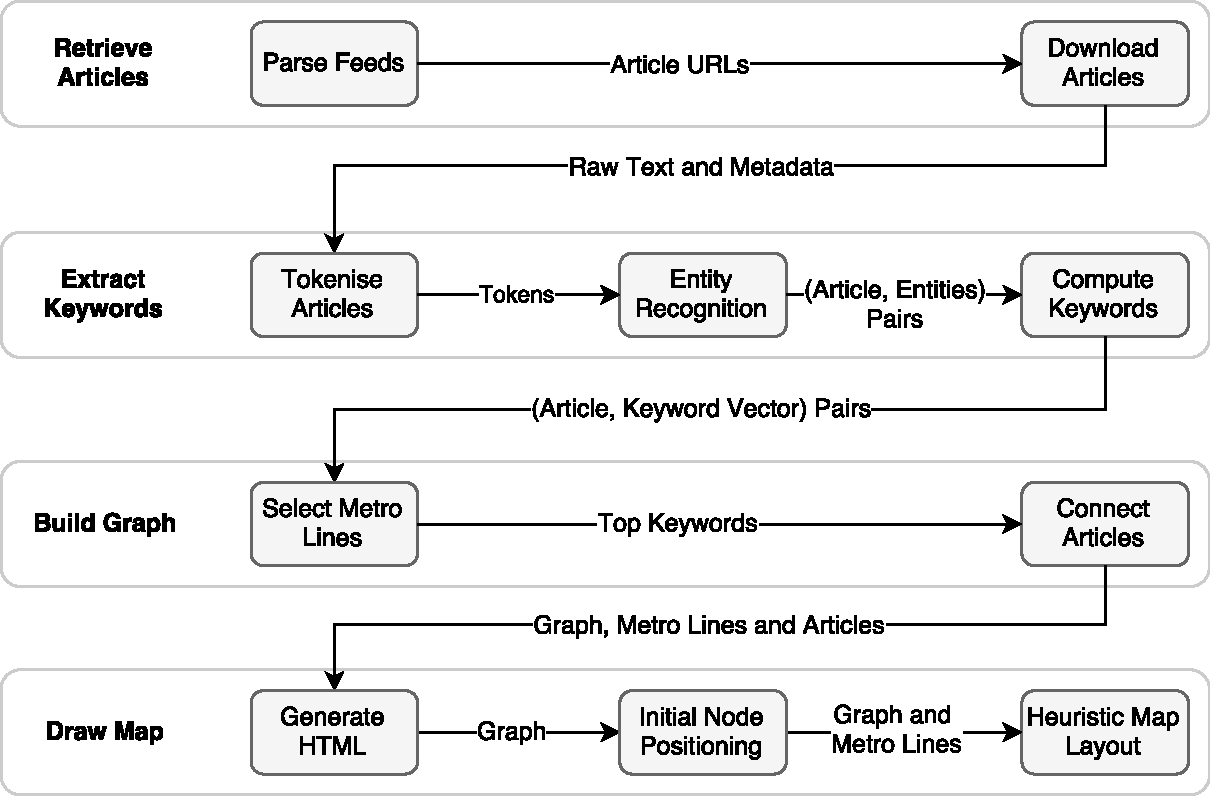
\includegraphics[width=\textwidth]{img/design/DataFlow.pdf}
	\caption{A conceptual model of data flow between components of the system.}
	\label{fig:dfp}
\end{figure}

Not included in Figure \ref{fig:dfp} is the boundary between the \textit{Build Graph} and \textit{Draw Map} stages of the pipeline, which marks the transition from the run-time Python which extracts and processes the article data, to JavaScript which only runs once the visualisation is opened in the browser; the entirety of the  \textit{Draw Map} stage. The boundary takes the form of an intermediate layer between \textit{Build Graph} and \textit{Draw Map}, where the topological map and the article data required for the visualisation are serialised to JSON\footnote{JavaScript Object Notation; \url{http://www.json.org}}.

\section{Discussion}

Central to the importance of the project is the knowledge that news consumers do not subscribe to single RSS feeds; they specifically seek out software which aggregates multiple feeds for convenience \citep{nreader}. Consequentially, \ref{f1.1} specifies that the system must accept multiple RSS feeds. However, news preferences are diverse, which gives rise to the potential case where a user specifies multiple feeds which do not share any significant keywords, and articles from one feed are excluded from the visualisation due to their lack of connectivity with the others. 

Initially, we considered a requirement for the connectivity \citep{GeneratingInformationMaps} of every metro line to be greater than one; that is, no line should be included in the visualisation unless it intersects with another. However, in the case described above, mutually exclusive RSS feeds could lead to `orphaned' lines which still contain useful content but do not share contextual links to the main body of the map. The stories on these lines should not be ignored by the system, as they most likely would not be ignored by a user browsing with a traditional RSS reader. Our argument is that the lack of connectivity of an article can itself be viewed as metadata on that article, and is not something to be penalised. However, a map which only contains orphaned lines is indicative of poor line selection, or--though this is less likely--a feed containing a set of completely unrelated articles. This highlights a fundamental assumption of the project; that in order to be of use, RSS feeds should contain explicitly related content.

A second issue of deliberation was the specification that stations on the generated maps should not be labelled (\ref{f4.7}). The use of node labels is logical for a search task, where locating a particular entity or route on a map is the goal. However, when the goal is gaining an insight into the structure of the collection being visualised, labelling each station with the title of the article it represents would only reintroduce the information overload we are attempting to mitigate. The \textit{overview} in the ``Overview first" clause of the information seeking mantra \citep{TheEyesHaveIt} is by definition the highest level of abstraction available on each data point, and while in a typical RSS reader this may well be the title, in our system this will not be the case. The context of the articles, that is, the metro lines themselves are what provide the overview, and the titles instead fall under ``details-on-demand."

One requirement which was left deliberately vague was (\ref{f4.8}); where possible, maps should comply with \possessivecite{AutomaticMetroMapLayoutThesis} aesthetic criteria for metro map layouts. The lack of strictness and specificity in this requirement was due to the non-spatial nature of the data being represented. While it is likely that there is an optimal layout for metro maps schematising real transit networks due to the geographic positioning of stations on those networks, there is no ``sensible'' underlying topology to metro maps of news to serve as a starting point. It was unknown at this stage whether we would be able to enforce strict layout criteria without significant pruning of the data.



